\setcounter{section}{4}

\section{Configuración del mecanismo de generación}

\subsection{Origen del generador}

La generación de código se realizó con \textbf{UmpleOnline}
(\url{https://try.umple.org}), la interfaz web oficial del compilador
Umple, desarrollado y mantenido por el laboratorio CRUISE de la
Universidad de Ottawa como proyecto de código abierto. Umple es un
lenguaje de modelado textual que permite expresar clases, atributos,
asociaciones y máquinas de estado, y transformarlos directamente a
código fuente en varios lenguajes destino, entre ellos Java, que es el
utilizado en este proyecto.

La versión exacta de la herramienta empleada fue verificada por dos
vías independientes, que reportan dos identificadores de build
distintos correspondientes a dos componentes separados de la
herramienta: (a) el pie de página de la interfaz web, que declara
\texttt{v1.37.0.8639.f07c3e9b7} y enlaza a la release correspondiente
en GitHub, y (b) el comentario de cabecera que el generador inserta
automáticamente en cada archivo \texttt{.java} producido, el cual
declara \texttt{1.37.0.8639.dcaf9c798} como versión del motor de
compilación Umple. Ambos identificadores comparten la misma versión
de release (\texttt{1.37.0.8639}) pero difieren en el \emph{hash} de
build porque corresponden a componentes distintos de UmpleOnline: la
interfaz web (front-end) y el motor de compilación que efectivamente
transforma el modelo en código Java. Se documentan ambos valores
--sin forzar su coincidencia-- para máxima trazabilidad, y ambos se
replicaron en el \texttt{README.md} del repositorio. Consultado el 20
de julio de 2026.

\subsection{Parámetros de generación}

Los parámetros aplicados al proceso de generación fueron los
siguientes:

\begin{itemize}
  \item \textbf{Lenguaje destino:} Java, mediante la opción
        \emph{Java Code} del menú \emph{Generate} de UmpleOnline.
  \item \textbf{Paquete de salida:} declarado en el propio modelo con
        la directiva \texttt{namespace ec.uteq.camaronera.piscinas;},
        situada como primera línea del archivo
        \texttt{modelo/camaronera.ump}. Esta directiva determina tanto
        la sentencia \texttt{package} de cada clase generada como la
        jerarquía de carpetas del código resultante.
  \item \textbf{Directorio de salida:} UmpleOnline no permite
        configurar la ruta de salida; el equipo adoptó como convención
        descargar el paquete comprimido mediante la opción
        \emph{Download Files} del panel \textsc{save \& load} y
        descomprimirlo en la carpeta \texttt{generado/} del
        repositorio, conservando el árbol de paquetes.
  \item \textbf{Convención de nombres:} impuesta por el generador y no
        editable. Umple produce sistemáticamente métodos con los
        patrones \texttt{getX}, \texttt{setX}, \texttt{addX},
        \texttt{removeX} y \texttt{numberOfX} según el tipo de miembro
        y la multiplicidad de cada asociación; el equipo la documenta
        como parámetro fijo de la herramienta.
  \item \textbf{Generadores no utilizados:} no se activó la generación
        SQL (\texttt{UmpleToSql}) por estar la persistencia fuera del
        alcance de este módulo, ni la generación de pruebas, que en
        Umple solo está disponible a través del compilador por línea
        de comandos y no desde el panel web. La verificación funcional
        se realiza mediante la unidad demostrable descrita en la
        Sección~6.2.
\end{itemize}

\paragraph{Política ante regeneración.}
El comportamiento de la herramienta ante una regeneración es la
\emph{sobrescritura completa} de las clases modeladas: el código Java
generado no incluye bloques protegidos que preserven ediciones
manuales. En consecuencia, el equipo adoptó la siguiente regla: está
prohibido editar cualquier archivo dentro de \texttt{generado/}; todo
cambio de dominio nace en \texttt{modelo/camaronera.ump} y se
regenera; el código escrito a mano (la clase de demostración
\texttt{DemoPiscinas.java}) vive exclusivamente en la carpeta
\texttt{manual/}, fuera del árbol regenerado, por lo que una
regeneración no tiene ningún efecto sobre él. El cumplimiento de esta
política es verificable por dos mecanismos: la cabecera
\emph{PLEASE DO NOT EDIT THIS CODE} presente en todo archivo generado,
y el historial de \emph{commits} del repositorio, donde cada
regeneración se registra como un cambio atómico sobre
\texttt{generado/}.

\subsection{Decisiones de mapeo}

La Tabla~3 resume las decisiones de mapeo entre las construcciones UML
del modelo y las construcciones Java producidas por el generador. Las
correspondencias principales son las siguientes: cada clase UML se
transforma en una clase Java homónima; cada atributo, en un campo
privado con sus métodos de acceso \texttt{getX}/\texttt{setX}; la
generalización (\texttt{isA} en Umple) se traduce en la cláusula
\texttt{extends}; y cada operación modelada conserva su firma en la
clase generada, junto con los métodos de infraestructura
\texttt{toString()} y \texttt{delete()} que Umple añade por defecto a
toda clase. Cabe precisar que Umple \emph{no} genera \texttt{equals()}
ni \texttt{hashCode()} salvo que se declare una clave (\texttt{key})
en la clase, recurso que este modelo no emplea.

En cuanto a las relaciones, el mapeo depende de la multiplicidad y del
tipo de asociación:

\begin{itemize}
  \item \textbf{Asociación \texttt{1 -- *} (Camaronera--Piscina y
        Piscina--CicloCultivo):} en el extremo ``uno'' se genera la
        colección con \texttt{getX()}, \texttt{numberOfX()} y el
        método \texttt{addX()}; en el extremo ``muchos'', una
        referencia obligatoria al padre, exigida en el constructor
        (\texttt{Piscina} exige su \texttt{Camaronera};
        \texttt{CicloCultivo} exige su \texttt{Piscina}).
  \item \textbf{Composición \texttt{1 <@>- *} / \texttt{1 <@>- 0..1}
        (CicloCultivo--Muestreo, CicloCultivo--Alimentacion y
        CicloCultivo--Cosecha):} el mismo mapeo anterior, más el
        método \texttt{delete()} del compuesto (\texttt{CicloCultivo})
        propagando la eliminación a sus tres tipos de parte (borrado
        en cascada).
  \item \textbf{Referencia obligatoria \texttt{* -- 1} (Muestreo--Empleado
        y Alimentacion--Insumo):} se genera un \texttt{setX()} que
        mantiene la integridad bidireccional del vínculo; no se genera
        \texttt{removeX()} en este extremo.
  \item \textbf{Multiplicidad mínima:} las restricciones de mínimo
        (extremos obligatorios) se exigen en los constructores y en
        tiempo de ejecución, no en tiempo de compilación.
\end{itemize}

Las directivas de Umple utilizadas y su efecto en el código Java se
resumen a continuación:

\begin{table}[h]
  \centering
  \caption{Directivas Umple empleadas y su traducción a Java.}
  \begin{tabular}{|l|p{8.5cm}|}
    \hline
    \textbf{Directiva Umple} & \textbf{Efecto en el código Java} \\
    \hline
    \texttt{namespace} &
      Sentencia \texttt{package} en cada clase y jerarquía de
      carpetas \texttt{ec/uteq/camaronera/piscinas/}. \\
    \hline
    \texttt{isA} &
      Cláusula \texttt{extends} (TecnicoCampo y Administrador heredan
      de Empleado). \\
    \hline
    \texttt{<@>-} (composición) &
      Borrado en cascada de las partes al invocar \texttt{delete()}
      sobre el compuesto. \\
    \hline
  \end{tabular}
\end{table}

El modelo no emplea \texttt{singleton}, \texttt{immutable},
\texttt{abstract}, \texttt{lazy} ni \emph{traits}: su ausencia es una
decisión de diseño ---el dominio del módulo no los requiere--- y no
una omisión de documentación, por lo que no aplican mapeos
adicionales.

\subsection{Archivos de configuración en el repositorio}

Dado que UmpleOnline no utiliza archivos de configuración externos,
la parametrización del proceso se documenta en el archivo
\texttt{plantillas/opciones-generacion.md} del repositorio, que
registra: (1) la herramienta, su URL y la versión exacta con fecha de
acceso; (2) la fuente única de generación, que es
\texttt{modelo/camaronera.ump} identificado por el \emph{hash} del
\emph{commit} correspondiente
(\texttt{0a2d178385b027df7bca755653b2804fbe7a812d}) ---el archivo no se duplica en otras
carpetas para evitar divergencias---; (3) la opción literal de
generación utilizada (\emph{Java Code}); (4) el \emph{namespace}
declarado; (5) los generadores descartados y su motivo; (6) la
política ante regeneración descrita en la Sección~5.2; y (7) el
procedimiento de exportación (\emph{Download Files}
$\rightarrow$ \texttt{generado/}). Con ello, cualquier miembro del
equipo o evaluador puede reproducir la generación en las mismas
condiciones.

\section{Proceso de generación y verificación del código}

\subsection{Ejecución de la generación}

El proceso se ejecutó en tres pasos, documentados con capturas de
pantalla almacenadas en \texttt{evidencias/capturas/}:

\begin{enumerate}
  \item \textbf{Edición y validación del modelo:} el archivo
        \texttt{camaronera.ump} se cargó en UmpleOnline, cuyo panel
        dividido muestra simultáneamente el modelo textual y el
        diagrama de clases renderizado sin errores de compilación del
        modelo (Figura~\ref{fig:panel-dividido}).
  \item \textbf{Generación y descarga:} se ejecutó \emph{Generate
        $\rightarrow$ Java Code} y se descargó el paquete completo
        mediante la opción \emph{Download Files} del panel
        \textsc{save \& load} (Figura~\ref{fig:descarga}).
  \item \textbf{Incorporación al repositorio:} el archivo comprimido
        se descomprimió en \texttt{generado/}, conservando el árbol de
        paquetes \texttt{ec/uteq/camaronera/piscinas/} con los diez
        archivos \texttt{.java} (Figura~\ref{fig:arbol-generado}).
\end{enumerate}

\begin{figure}[h]
  \centering
  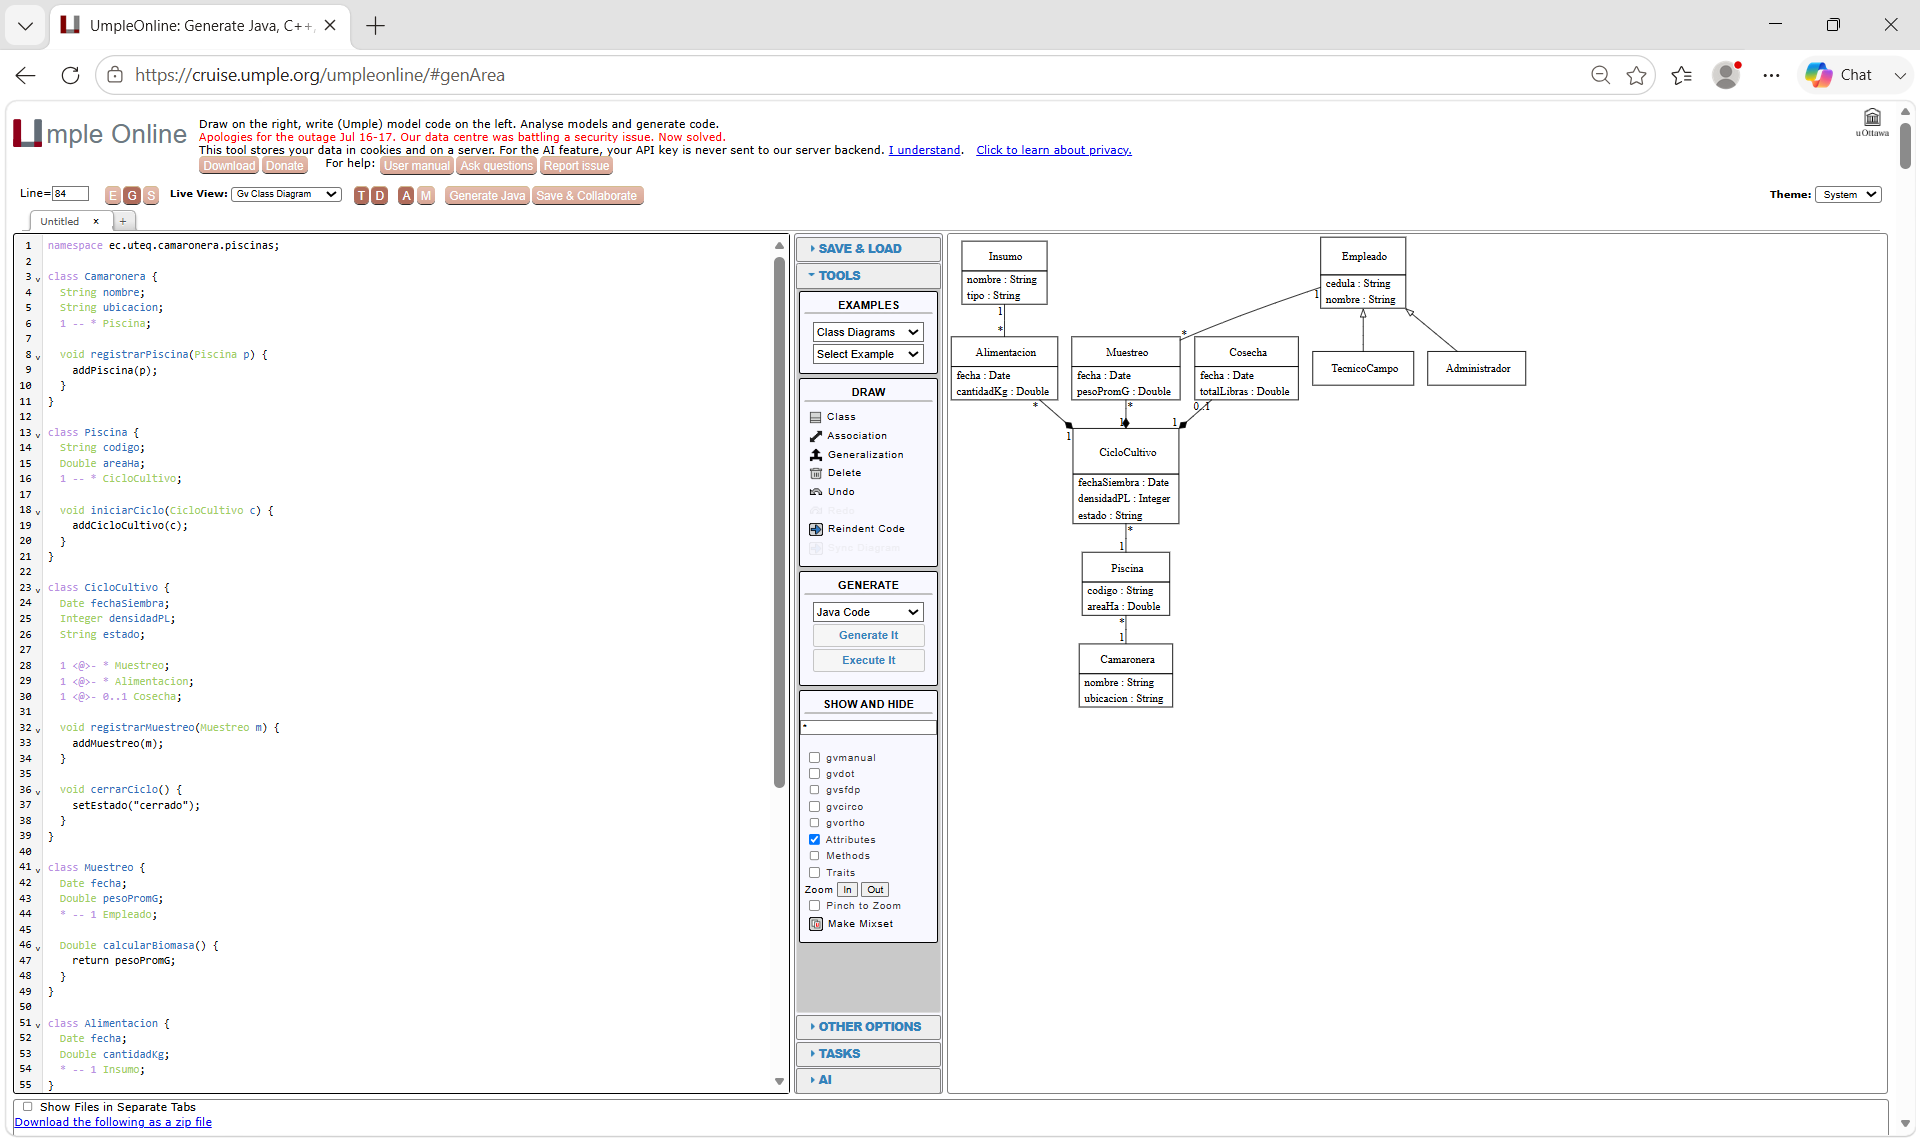
\includegraphics[width=0.85\textwidth]{../evidencias/capturas/01-panel-dividido.png}
  \caption{Panel dividido de UmpleOnline: modelo textual (izquierda) y
  diagrama de clases renderizado sin errores (derecha).}
  \label{fig:panel-dividido}
\end{figure}

\begin{figure}[h]
  \centering
  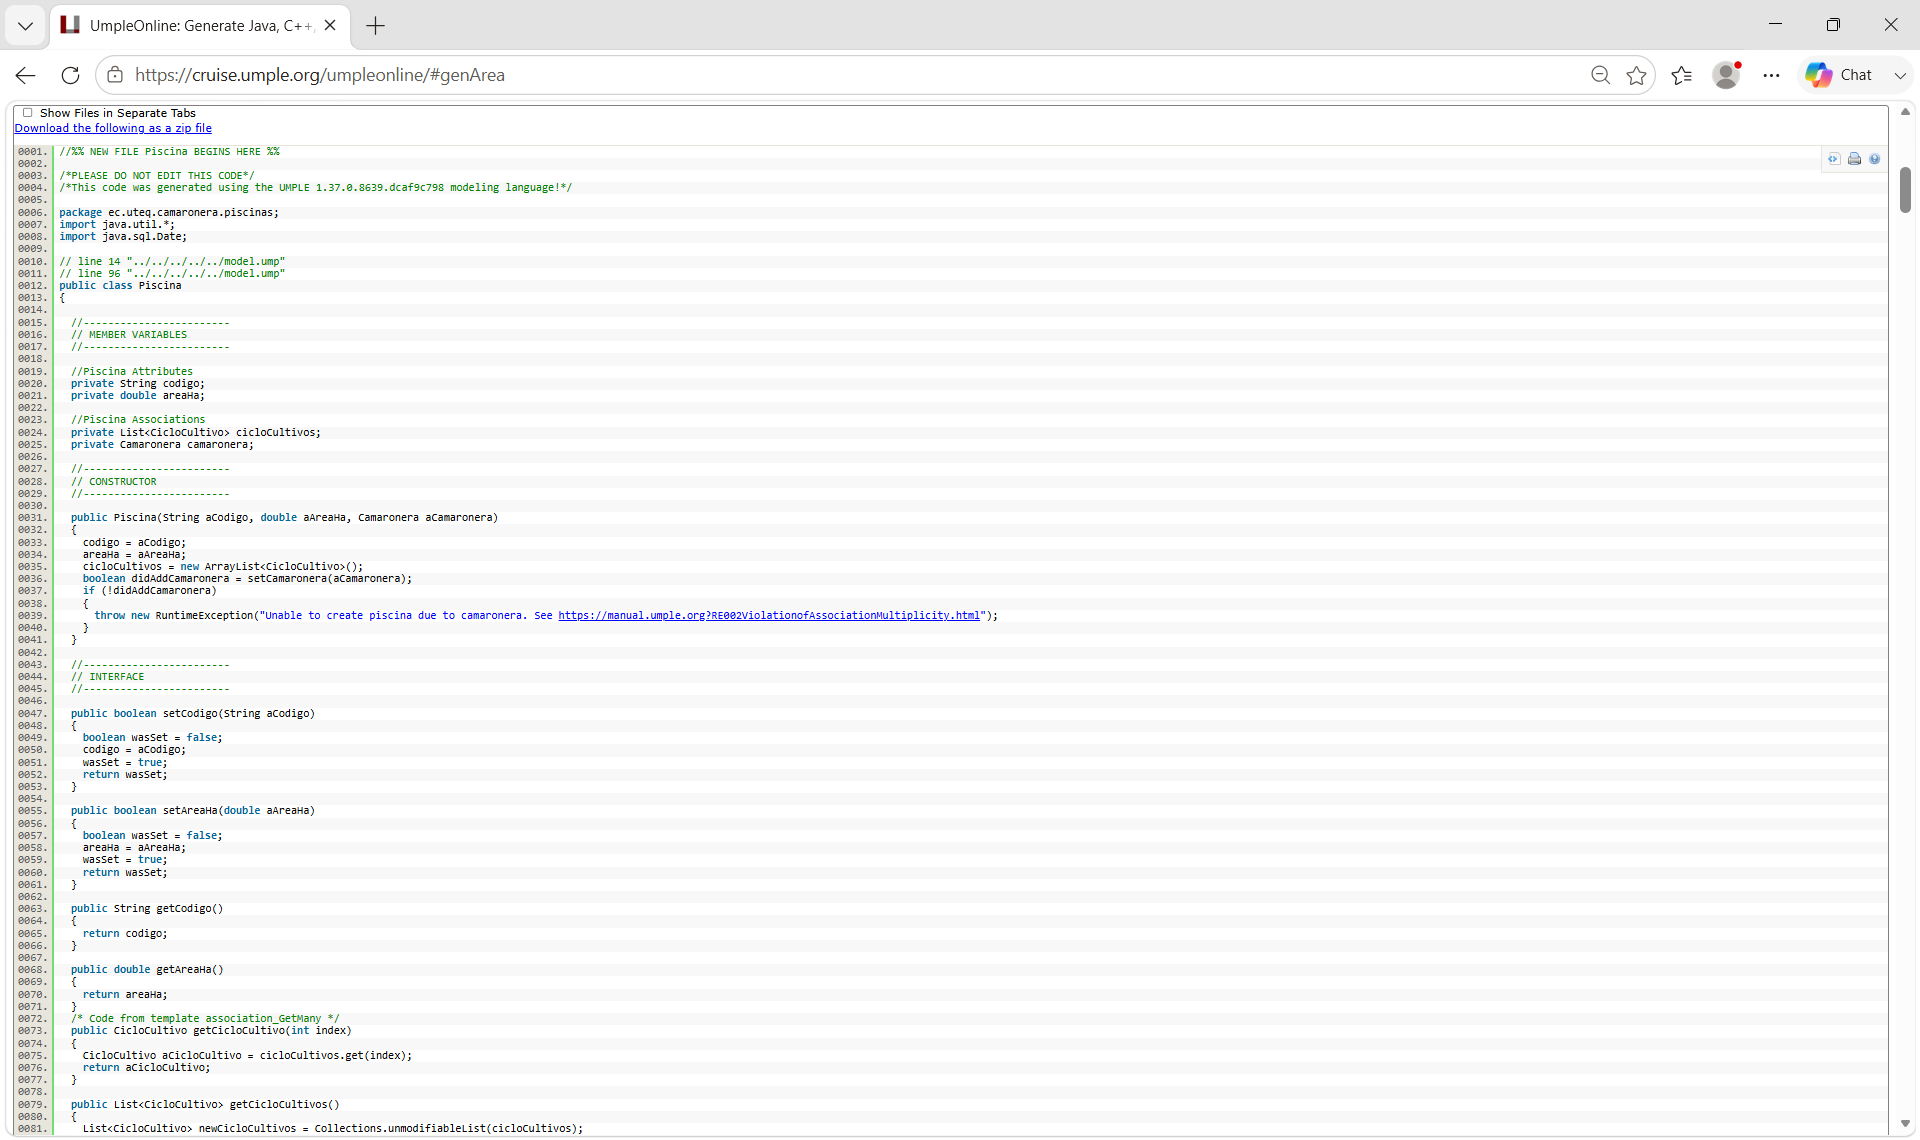
\includegraphics[width=0.85\textwidth]{../evidencias/capturas/02-descarga.png}
  \caption{Resultado de \emph{Generate $\rightarrow$ Java Code}: código
  Java generado (clase \texttt{Piscina}) con cabecera
  \emph{PLEASE DO NOT EDIT THIS CODE} y versión del motor Umple.}
  \label{fig:descarga}
\end{figure}

\begin{figure}[h]
  \centering
  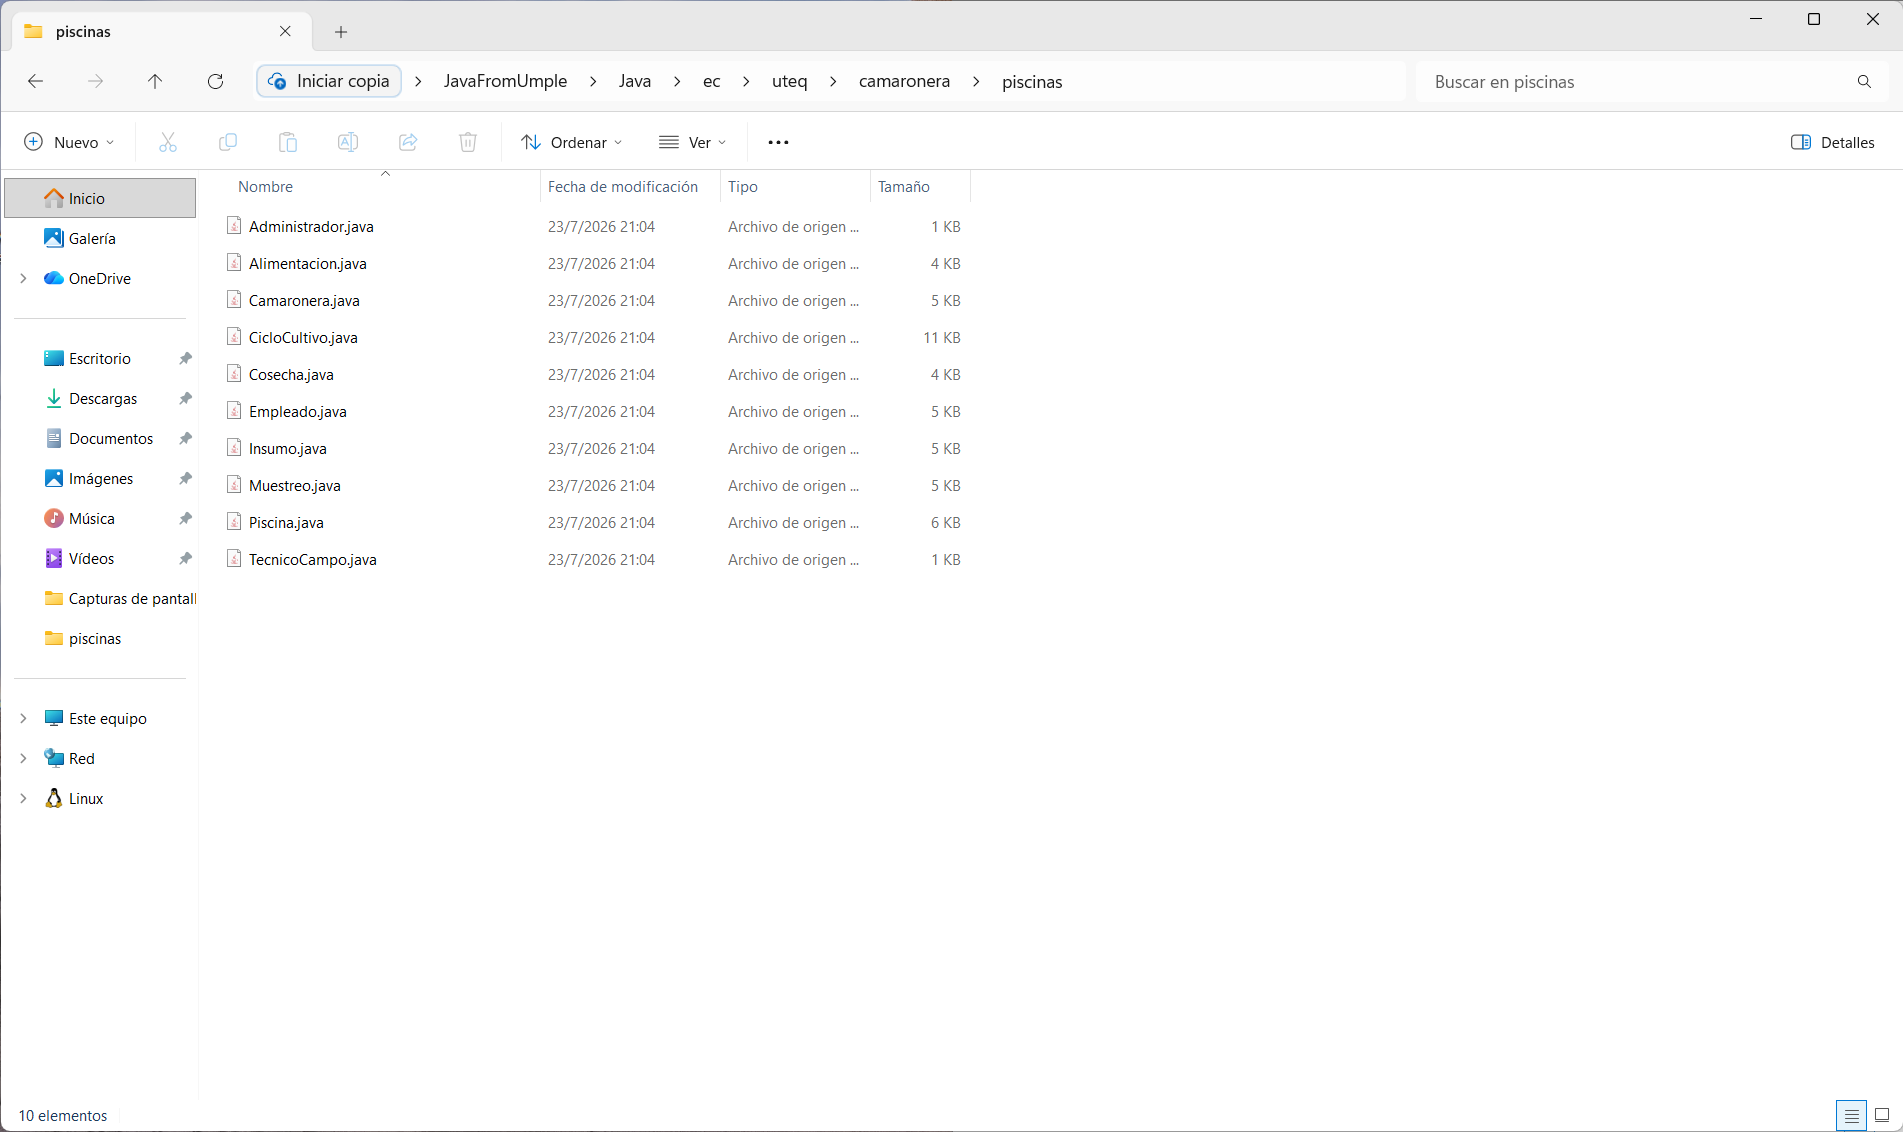
\includegraphics[width=0.85\textwidth]{../evidencias/capturas/03-arbol-generado.png}
  \caption{Árbol de archivos generados en \texttt{generado/ec/uteq/camaronera/piscinas/}:
  los diez archivos \texttt{.java} correspondientes a las diez clases del modelo.}
  \label{fig:arbol-generado}
\end{figure}

\paragraph{Coherencia entre la estructura del proyecto y el modelo.}
La estructura resultante es coherente con el modelo por tres
evidencias verificables. Primera, existe una correspondencia uno a uno
entre las diez clases del modelo y los diez archivos generados, de
nombre idéntico, como muestra la captura del árbol y la columna de
archivos de la Tabla~\ref{tab:correspondencia}. Segunda, la jerarquía de carpetas reproduce
exactamente el \emph{namespace} declarado, que a su vez representa el
subsistema modelado (módulo de piscinas del sistema de la
camaronera). Tercera, el inventario del paquete descargado no contiene
archivos adicionales sin clasificar: todo su contenido corresponde a
clases del modelo.

\paragraph{Distinción entre código generado y código manual.}
El repositorio permite distinguir de forma objetiva el código generado
del escrito a mano mediante tres mecanismos simultáneos: (a) la
separación física en carpetas, pues \texttt{generado/} contiene
exclusivamente la salida de la herramienta y \texttt{manual/} el único
archivo escrito por el equipo (\texttt{DemoPiscinas.java}); (b) el
marcador del propio generador, ya que todo archivo producido por Umple
inicia con el comentario \emph{PLEASE DO NOT EDIT THIS CODE}, que
además declara la versión utilizada, marca ausente en el código
manual; y (c) la declaración explícita del código manual en el
\texttt{README.md} del repositorio y en esta sección.

\subsection{Compilación y ejecución de una unidad demostrable}

Como unidad demostrable se escribió la clase
\texttt{manual/ec/uteq/camaronera/piscinas/DemoPiscinas.java}, que
instancia el núcleo del dominio ---una camaronera con una piscina, un
ciclo de cultivo activo y un muestreo registrado por un empleado--- y
verifica mediante la API generada que el vínculo entre el ciclo y su
muestreo quedó establecido. El fragmento central es el siguiente
(las firmas de los constructores corresponden a las generadas por
Umple, que exigen los extremos de asociación obligatorios):

\begin{verbatim}
Empleado empleado = new Empleado("0912345678", "Juan Pérez");
Camaronera camaronera = new Camaronera("AquaGest", "Quevedo");
Piscina piscina = new Piscina("P-01", 2.5, camaronera);
CicloCultivo ciclo = new CicloCultivo(fechaSiembra, 12, "activo", piscina);
Muestreo muestreo = new Muestreo(fechaMuestreo, 8.5, empleado, ciclo);
System.out.println("Muestreos del ciclo: "
    + ciclo.getMuestreos().size());
\end{verbatim}

La compilación y ejecución se realizaron desde la raíz del
repositorio con los siguientes comandos:

\begin{verbatim}
javac -d out generado/ec/uteq/camaronera/piscinas/*.java \
      manual/ec/uteq/camaronera/piscinas/DemoPiscinas.java
java -cp out ec.uteq.camaronera.piscinas.DemoPiscinas
\end{verbatim}

La salida obtenida fue \texttt{Muestreos del ciclo: 1}, que confirma
que el código generado compila sin errores y que la asociación
CicloCultivo--Muestreo funciona conforme al modelo. La evidencia de la
compilación y de la salida en consola se encuentra en
\texttt{evidencias/capturas/} (Figura~\ref{fig:compilacion-salida}).

\begin{figure}[h]
  \centering
  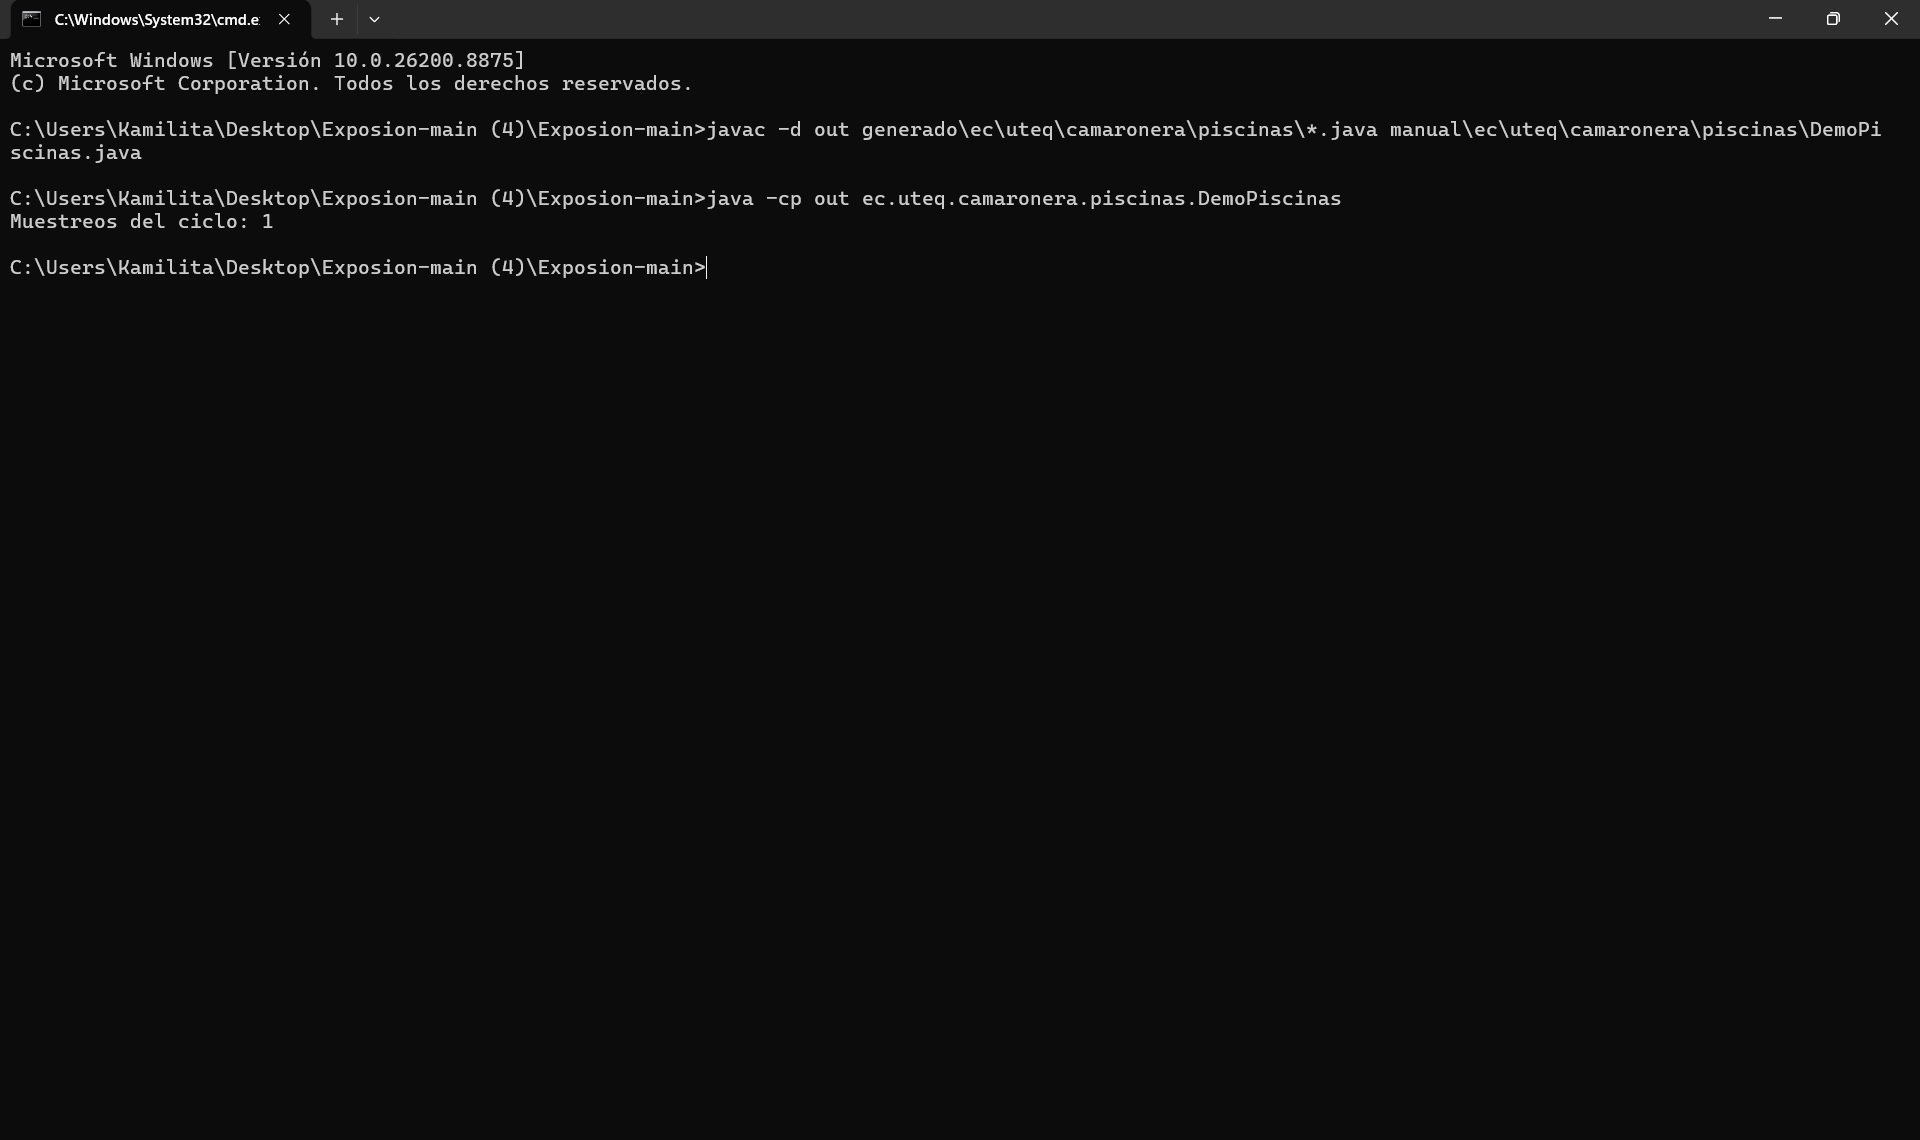
\includegraphics[width=0.85\textwidth]{../evidencias/capturas/04-compilacion-salida.png}
  \caption{Terminal mostrando la compilación sin errores y la ejecución
  de \texttt{DemoPiscinas}, con la salida \texttt{Muestreos del ciclo: 1}.}
  \label{fig:compilacion-salida}
\end{figure}

\subsection{Correspondencia entre el modelo y el código generado}

La Tabla~\ref{tab:correspondencia} documenta, clase por clase, la correspondencia entre los
elementos del modelo y el código generado: el archivo \texttt{.java}
resultante, la firma del constructor ---incluidos los extremos de
asociación obligatorios que el generador exige---, y los métodos de
asociación producidos según la multiplicidad de cada relación
(\texttt{addX()}/\texttt{getX()}/\texttt{numberOfX()} en los extremos
de colección, \texttt{setX()} con integridad bidireccional en las
referencias obligatorias, y \texttt{delete()} con propagación en
cascada en las composiciones declaradas). Todos los nombres de la
tabla fueron confirmados contra el código efectivamente descargado,
de modo que la correspondencia es verificable abriendo cualquiera de
los archivos de \texttt{generado/} durante la exposición.

\begin{table}[h]
  \centering
  \caption{Correspondencia entre las clases del modelo y el código Java generado.}
  \label{tab:correspondencia}
  \small
  \begin{tabular}{|l|l|p{6.3cm}|}
    \hline
    \textbf{Clase UML} & \textbf{Archivo generado} & \textbf{Constructor y métodos de asociación destacados} \\
    \hline
    Camaronera &
      \texttt{Camaronera.java} &
      \texttt{Camaronera(nombre, ubicacion)}; colección \texttt{piscinas} con \texttt{addPiscina()}, \texttt{getPiscinas()}, \texttt{numberOfPiscinas()}; \texttt{delete()} en cascada sobre sus piscinas. \\
    \hline
    Piscina &
      \texttt{Piscina.java} &
      \texttt{Piscina(codigo, areaHa, camaronera)} exige \texttt{camaronera} (lanza \texttt{RuntimeException} si es nula); colección \texttt{cicloCultivos}; \texttt{setCamaronera()} mantiene integridad bidireccional. \\
    \hline
    CicloCultivo &
      \texttt{CicloCultivo.java} &
      \texttt{CicloCultivo(fechaSiembra, densidadPL, estado, piscina)} exige \texttt{piscina}; colecciones \texttt{muestreos} y \texttt{alimentacions}; referencia opcional \texttt{cosecha} vía \texttt{setCosecha()} (patrón \emph{SetOptionalOneToOne}); \texttt{delete()} propaga a muestreos, alimentaciones y cosecha. \\
    \hline
    Muestreo &
      \texttt{Muestreo.java} &
      \texttt{Muestreo(fecha, pesoPromG, empleado, cicloCultivo)} exige ambos extremos; método de dominio \texttt{calcularBiomasa()}. \\
    \hline
    Alimentacion &
      \texttt{Alimentacion.java} &
      \texttt{Alimentacion(fecha, cantidadKg, insumo, cicloCultivo)} exige ambos extremos. \\
    \hline
    Cosecha &
      \texttt{Cosecha.java} &
      \texttt{Cosecha(fecha, totalLibras, cicloCultivo)}; \texttt{setCicloCultivo()} usa patrón \emph{SetOneToOptionalOne}: si el ciclo ya tiene otra cosecha asignada, rechaza el cambio para no huérfanar la existente. \\
    \hline
    Insumo &
      \texttt{Insumo.java} &
      \texttt{Insumo(nombre, tipo)}; colección \texttt{alimentacions} con \texttt{addAlimentacion()}. \\
    \hline
    Empleado &
      \texttt{Empleado.java} &
      \texttt{Empleado(cedula, nombre)}; colección \texttt{muestreos}; superclase de \texttt{TecnicoCampo} y \texttt{Administrador}. \\
    \hline
    TecnicoCampo &
      \texttt{TecnicoCampo.java} &
      \texttt{extends Empleado}; \texttt{TecnicoCampo(cedula, nombre)} delega en \texttt{super()}; método de rol \texttt{registrarMuestreo()} (cuerpo delegado, sin implementación de negocio). \\
    \hline
    Administrador &
      \texttt{Administrador.java} &
      \texttt{extends Empleado}; \texttt{Administrador(cedula, nombre)} delega en \texttt{super()}; método de rol \texttt{crearCiclo()} (cuerpo delegado). \\
    \hline
  \end{tabular}
\end{table}

\subsection{Limitaciones observadas del generador}

Durante el uso del generador se identificaron las siguientes
limitaciones, cada una con su evidencia y la estrategia adoptada:

\begin{table}[h]
  \centering
  \caption{Limitaciones observadas del generador y mitigación.}
  \begin{tabular}{|p{4.2cm}|p{4.6cm}|p{4.6cm}|}
    \hline
    \textbf{Limitación} & \textbf{Evidencia} & \textbf{Mitigación} \\
    \hline
    Los \emph{getters} de asociación devuelven listas inmutables;
    modificarlas directamente lanza
    \texttt{UnsupportedOperationException}. &
    Cuerpos de operación que usaban
    \texttt{getX().add(y)} fallaban en ejecución. &
    Usar siempre los métodos generados \texttt{addX()} en los cuerpos
    modelados en el \texttt{.ump}. \\
    \hline
    Los constructores exigen los extremos de asociación obligatorios,
    lo que impone un orden de creación de objetos. &
    Firmas de los constructores en
    \texttt{generado/}. &
    Documentar el orden de instanciación en la unidad demostrable
    (Sección~6.2). \\
    \hline
    Las multiplicidades mínimas se verifican en tiempo de ejecución,
    no en compilación. &
    Violaciones de mínimo producen fallos al ejecutar, no al
    compilar. &
    Cubrir los escenarios de creación en la unidad demostrable y en
    las pruebas del PFC. \\
    \hline
    El generador no valida reglas de negocio del dominio (rangos de
    oxígeno, fechas coherentes, etc.). &
    El código generado acepta cualquier valor en los atributos. &
    Las validaciones de dominio se implementarán en la capa de
    servicios del PFC. \\
    \hline
    No hay bloques protegidos: la regeneración sobrescribe todo el
    código generado. &
    Cabecera \emph{PLEASE DO NOT EDIT THIS CODE} en cada archivo. &
    Política de regeneración de la Sección~5.2 (código manual fuera
    de \texttt{generado/}). \\
    \hline
    La generación de pruebas no está disponible en el panel web,
    solo mediante el compilador por línea de comandos. &
    Menú \emph{Generate} de UmpleOnline sin opción de pruebas. &
    Verificación funcional mediante la unidad demostrable
    \texttt{DemoPiscinas}. \\
    \hline
    UmpleOnline no permite configurar el directorio de salida. &
    La descarga entrega un único archivo comprimido. &
    Convención de equipo: descompresión en \texttt{generado/}
    (Sección~5.2). \\
    \hline
  \end{tabular}
\end{table}

Estas limitaciones no comprometen el objetivo del ciclo MDD: el
código de dominio se obtiene íntegramente del modelo, y los aspectos
no cubiertos por el generador quedan explícitamente asignados a
etapas posteriores del proyecto.

